\documentclass[10pt,a4paper]{article}
\usepackage[T1]{fontenc}
\usepackage[brazil]{babel}
\usepackage[utf8]{inputenc}


\usepackage{ae,aecompl}
\usepackage{pslatex}
\usepackage{epsfig}
\usepackage{geometry}
\usepackage{url}
\usepackage{textcomp}
\usepackage{ae}
\usepackage{subfig}
\usepackage{indentfirst}
\usepackage{textcomp}
\usepackage{color}
\usepackage{setspace}
\usepackage{verbatim}
\usepackage{mathtools}
\usepackage{amsmath}


\linespread{1.5}
\geometry{ 
	a4paper,	% Formato do papel
	tmargin=30mm,	% Margem superior
	bmargin=40mm,	% Margem inferior
	lmargin=20mm,	% Margem esquerda
	rmargin=20mm,	% Margem direita
	footskip=20mm	% Espaço entre o rodapé e o fim do texto
}
%  ABACO -- Conjunto de macros para desenhar o 'abaco

%  Desenho original de Hans Liesenberg

%  Macros de Tomasz Kowaltowski

%  DCC -- IMECC -- UNICAMP

%  Mar,co de 1988  --  Vers~ao 1.0

% Ajustado para LaTeX da SUN -- Mar,co de 1991

% ---------------------------------------------------------

%  Chamada:   \ABACO{d1}{d2}{d3}{d4}{esc}
%             com:  di's -- os quatro d'igitos;
%	           esc  -- fator de escala

% ---------------------------------------------------------

%  DEFINI,C~OES AUXILIARES

% ---------------------------------------------------------


%  Forma o d'igito pequeno (0 ou 1)

\newcommand{\ABACODP}[1]{%
%
\thicklines
%    
\begin{picture}(8,0)
    \ifcase#1{   %  caso 0
       \put(0,0)    {\line(1,0){4}}
       \multiput(5,0)(2,0){2}{\oval(2,4)}}
    \or{         %  caso 1
       \put(2,0)    {\line(1,0){4}}
       \multiput(1,0)(6,0){2}{\oval(2,4)}}
    \fi
\end{picture}
    } % \ABACODP

% Forma o d'igito grande (0 a 4)

\newcommand{\ABACODG}[1]{%
%
\thicklines
%    
\begin{picture}(14,0)
    \ifcase#1{   % caso 0
       \multiput(1,0)(2,0){5}{\oval(2,4)}}
       \put(10,0)   {\line(1,0){4}}
    \or{         % caso 1
       \multiput(1,0)(2,0){4}{\oval(2,4)}}
       \put(8,0)   {\line(1,0){4}}
       \put(13,0)   {\oval(2,4)}
    \or{         % caso 2
       \multiput(1,0)(2,0){3}{\oval(2,4)}
       \put(6,0)   {\line(1,0){4}}
       \multiput(11,0)(2,0){2}{\oval(2,4)}}
    \or{         % caso 3
       \multiput(1,0)(2,0){2}{\oval(2,4)}
       \put(4,0)   {\line(1,0){4}}
       \multiput(9,0)(2,0){3}{\oval(2,4)}}
    \or{         % caso 4
       \put(1,0)  {\oval(2,4)}}
       \put(2,0)   {\line(1,0){4}}
       \multiput(7,0)(2,0){4}{\oval(2,4)}
    \fi
\end{picture}
    } % \ABACODG
       
% Forma um d'igito (0 a 9)

\newcommand{\ABACOD}[1]{%
%
    \ifnum#1>9
       \errmessage{#1: Argumento invalido para ABACO}
    \fi
    \ifnum#1<0
       \errmessage{#1: Argumento invalido para ABACO}
    \fi
%
\begin{picture}(24,0)
%    
    \ifnum#1<5
       \put(16,0) {\ABACODP{0}}
    \else   
       \put(16,0) {\ABACODP{1}}
    \fi
%    
    \ifnum#1<5
       \put(0,0)  {\ABACODG{#1}}
    \else
       \ifcase#1\or \or \or \or
          \or  \put(0,0)  {\ABACODG{0}}
          \or  \put(0,0)  {\ABACODG{1}}
          \or  \put(0,0)  {\ABACODG{2}}
          \or  \put(0,0)  {\ABACODG{3}}
          \or  \put(0,0)  {\ABACODG{4}}
       \fi
    \fi   
\end{picture}
    } % \ABACOD
    
% -------------------------------------------------

%  DEFINI,C~AO PRINCIPAL
    
\newcommand{\ABACO}[5]{%
    \setlength{\unitlength}{#5mm}
%
    \thinlines
%   
\begin{picture}(28,25)
%   
% moldura
%
% externa
%
        \put(0,0)            {\line(0,1){25}}
        \put(0,0)            {\line(1,0){28}}
        \put(28,0)           {\line(0,1){25}}
        \put(0,25)           {\line(1,0){28}}
% interna
        \put(2,2)            {\line(0,1){21}}
	\put(26,2)           {\line(0,1){21}}
	\put(16,2)           {\line(0,1){21}}
	\put(18,2)           {\line(0,1){21}}
	\put(2,2)            {\line(1,0){14}}
	\put(16,2)           {\line(1,-1){1}}
	\put(17,1)           {\line(1,1){1}}
	\put(18,2)           {\line(1,0){8}}
	\put(2,23)           {\line(1,0){14}}
	\put(16,23)          {\line(1,1){1}}
	\put(17,24)          {\line(1,-1){1}}
	\put(18,23)          {\line(1,0){8}}
	\put(0,0)            {\line(1,1){2}}
	\put(0,25)           {\line(1,-1){2}}
	\put(28,0)           {\line(-1,1){2}}
	\put(28,25)          {\line(-1,-1){2}}
%
%   
% d'igitos
%
%   
       \put(2,20)  {\ABACOD{#1}}
       \put(2,15)  {\ABACOD{#2}}
       \put(2,10)  {\ABACOD{#3}}
       \put(2,5)   {\ABACOD{#4}}
%      
\end{picture}
    } % \ABACO
    
 
\renewcommand{\thetable}{\Roman{table}}
\newcommand{\x} {$\bullet$}


\begin{document}
% CAPA
\begin{titlepage}
\thispagestyle{empty}
  \begin{center} {\large \textbf{UNIVERSIDADE~ESTADUAL~DE~CAMPINAS}} \end{center}
  \begin{center} {\large INSTITUTO~DE~COMPUTAÇÃO}                    \end{center}
  \vspace{0.1cm}
  \begin{center}
  \begin{minipage}[tl]{31mm}
    \ABACO{1}{9}{6}{9}{1}
  \end{minipage}
  \end{center}
  \vspace{0.3cm}
  \begin{center} 
    {\large \textsc{São totalmente válidas algumas das considerações sobre a
Correlação de Pearson presentes na literatura?  }} 
    \\\vspace{0.5cm}
    {\textsl{Relatório do primeiro laboratório de MC920}}
    \\\vspace{1cm}
    \begin{tabular}{rl}
	  \textbf{Aluno}:   Carlos~Eduardo~Machado &  
	  \textbf{RA}:          059582 \\ 
	  \textbf{Aluno}:        Tiago~Chedraoui~Silva & 
	  \textbf{RA}:        082941 \\
	  \textbf{Aluno}:        William~Marques~Dias & 
	  \textbf{RA}:        065106 \\
	\end{tabular}
  \end{center}
  \vspace{0.5cm}

  \begin{abstract}
O coeficiente de correlação de Pearson é amplamente usado para
comparar imagens, contudo ele apresenta sérias limitações. Esse
trabalho consistiu na validação da análise realizada no Artigo ''The
Ineffectiveness of the Correlation Coefficient for Image Comparisons''.
  \end{abstract}
  % Sumário
  \tableofcontents
\end{titlepage} 

\vspace{2mm}
\newpage

\section{Introdução}
O coeficiente de correlação de Pearson é amplamente amplamente
utilizado na análise estatística, reconhecimento de padrões e
processamento de imagens.
Na área de processamento de imagens ele é utilizado na comparação de
duas imagens para fins de registro de imagens, reconhecimento de
objetos, e medição disparidade ~\cite{paper}. Para imagens digitais monocromáticas, a correlação de Pearson é definido como :

\begin{equation}r = \frac{  
\displaystyle{\sum_{i} (x_i-\bar{x})(y_i-  
\bar{y})}}{\displaystyle{\left[  
\sum_{i}(x_i-\bar{x})^2  
\sum_{i}(y_i-\bar{y})^2\right]^{1/2}}}  
\end{equation}  

Onde $x_i$ é a intensidade dos pixels na imagem 1, $y_i$ é a
intensidade dos pixels na imagem 2,$\bar{x}$ é a intensidade média da
imagem 1 e $\bar{y}$ é a intensidade média da imagem 2.

O coeficiente tem valor $r=1$ se as duas imagens são absolutamente
idênticas, $r=0$ se são totalmente não correlacionadas e $r=-1$ se elas
são totalmente anti-correlacionadas, por exemplo se uma imagem é o
negativo da outra.

O coeficiente de Pearson pode ser utilizado em
aplicações de segurança, como, por exemplo, vigilância. Normalmente, 
o coeficiente de relação é usado para comparar duas imagens do mesmo
objeto ou cena durante vários momentos diferentes.

O objetivo deste trabalho é apresentar, através de exemplos, o
desempenho do coeficiente para comparações de imagens, especialmente
em aplicações de segurança.

\section{Métodos}



\subsection{Código}

\newpage
\section{Resultados}
\begin{figure}[h!]
\begin{center}
\subfloat[Imagem original]{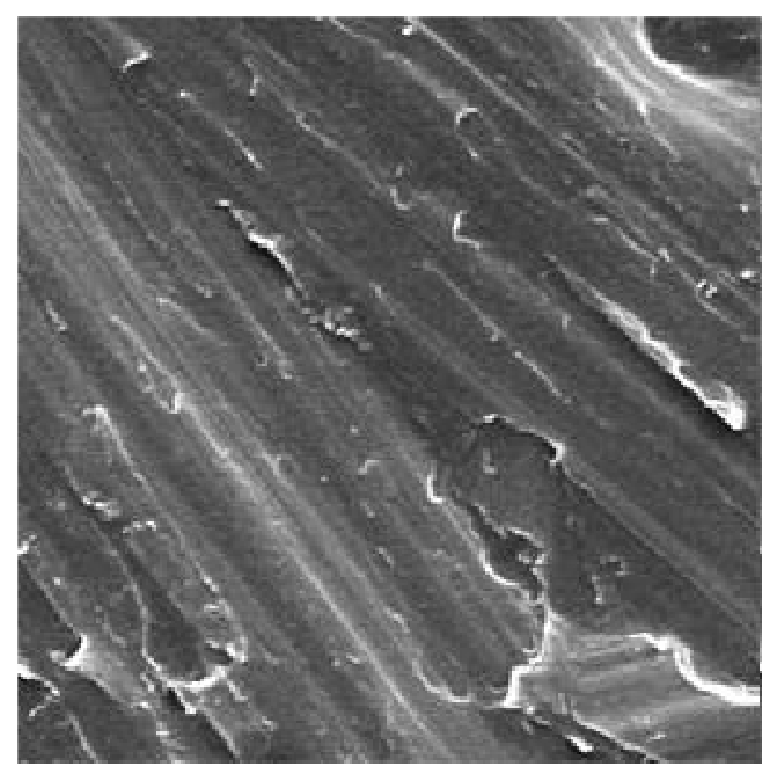
\includegraphics[scale=0.45]{photos/c1a}\label{
cacheDados}}
\hspace{10mm}
\subfloat[Sobreposição de uma palavra sobre a imagem]{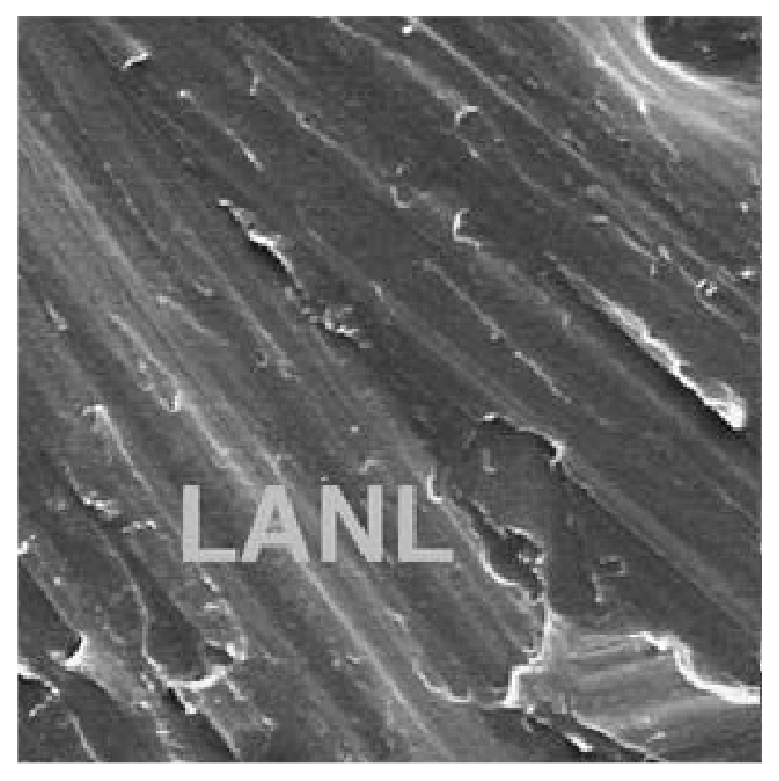
\includegraphics[scale=0.45]{photos/c1b}\label{cacheIns}}
\caption{Comparação entre uma imagem original e outra com sobreposição
  de palavra}
\end{center}
\end{figure}


%figura clipes

\begin{figure}[h!]
\begin{center}
\subfloat[Original]{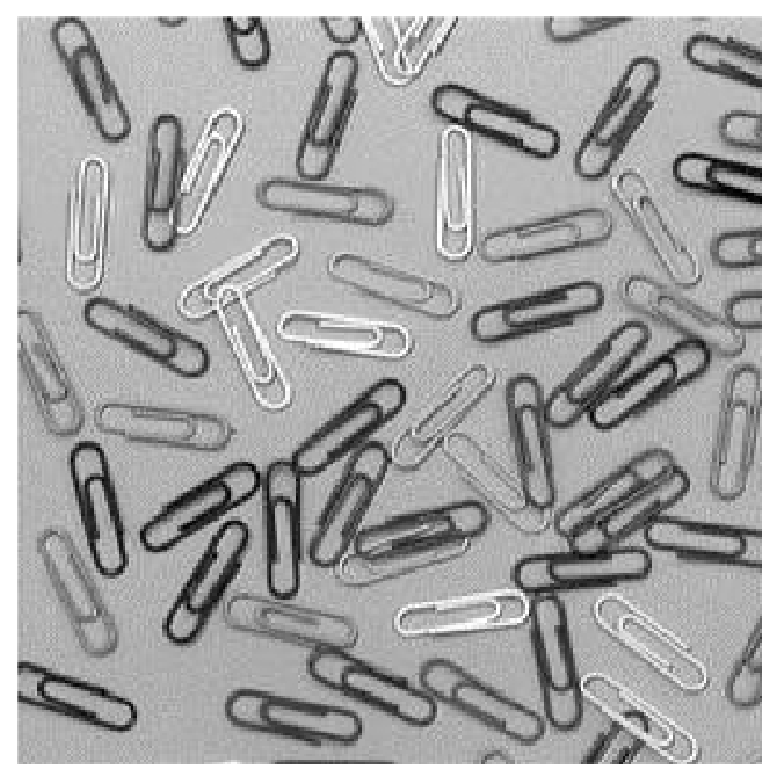
\includegraphics[scale=0.45]{photos/c2a}\label{
cacheDados}}
\hspace{10mm}
\subfloat[Remoção de um clipe na imagem original]{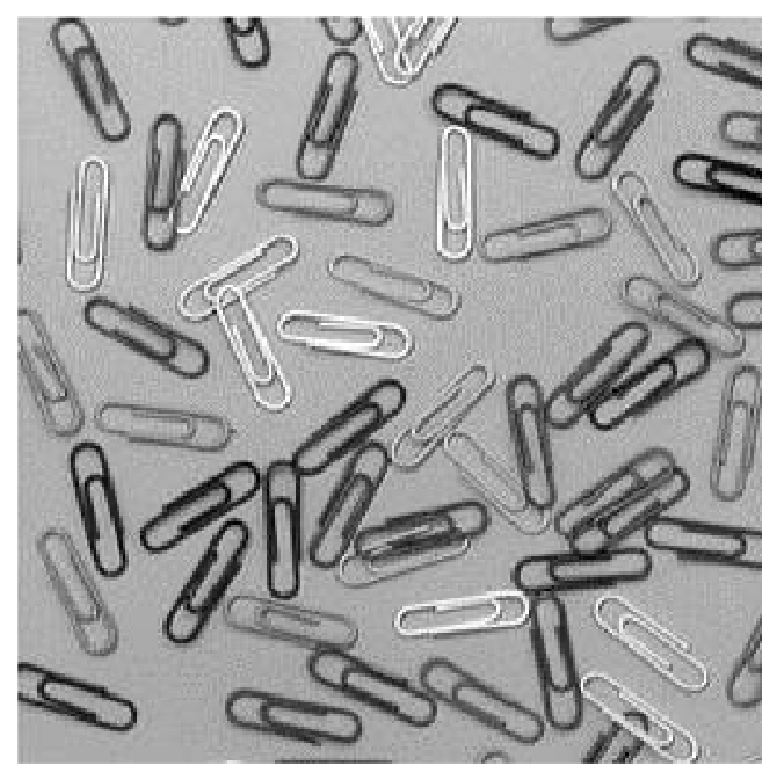
\includegraphics[scale=0.45]{photos/c2b}\label{cacheIns}}
\caption{Comparação entre imagem com um objeto e outra sem esse objeto}
\end{center}
\end{figure}

\newpage
%m15 fig1
\begin{figure}[h!]
\begin{center}
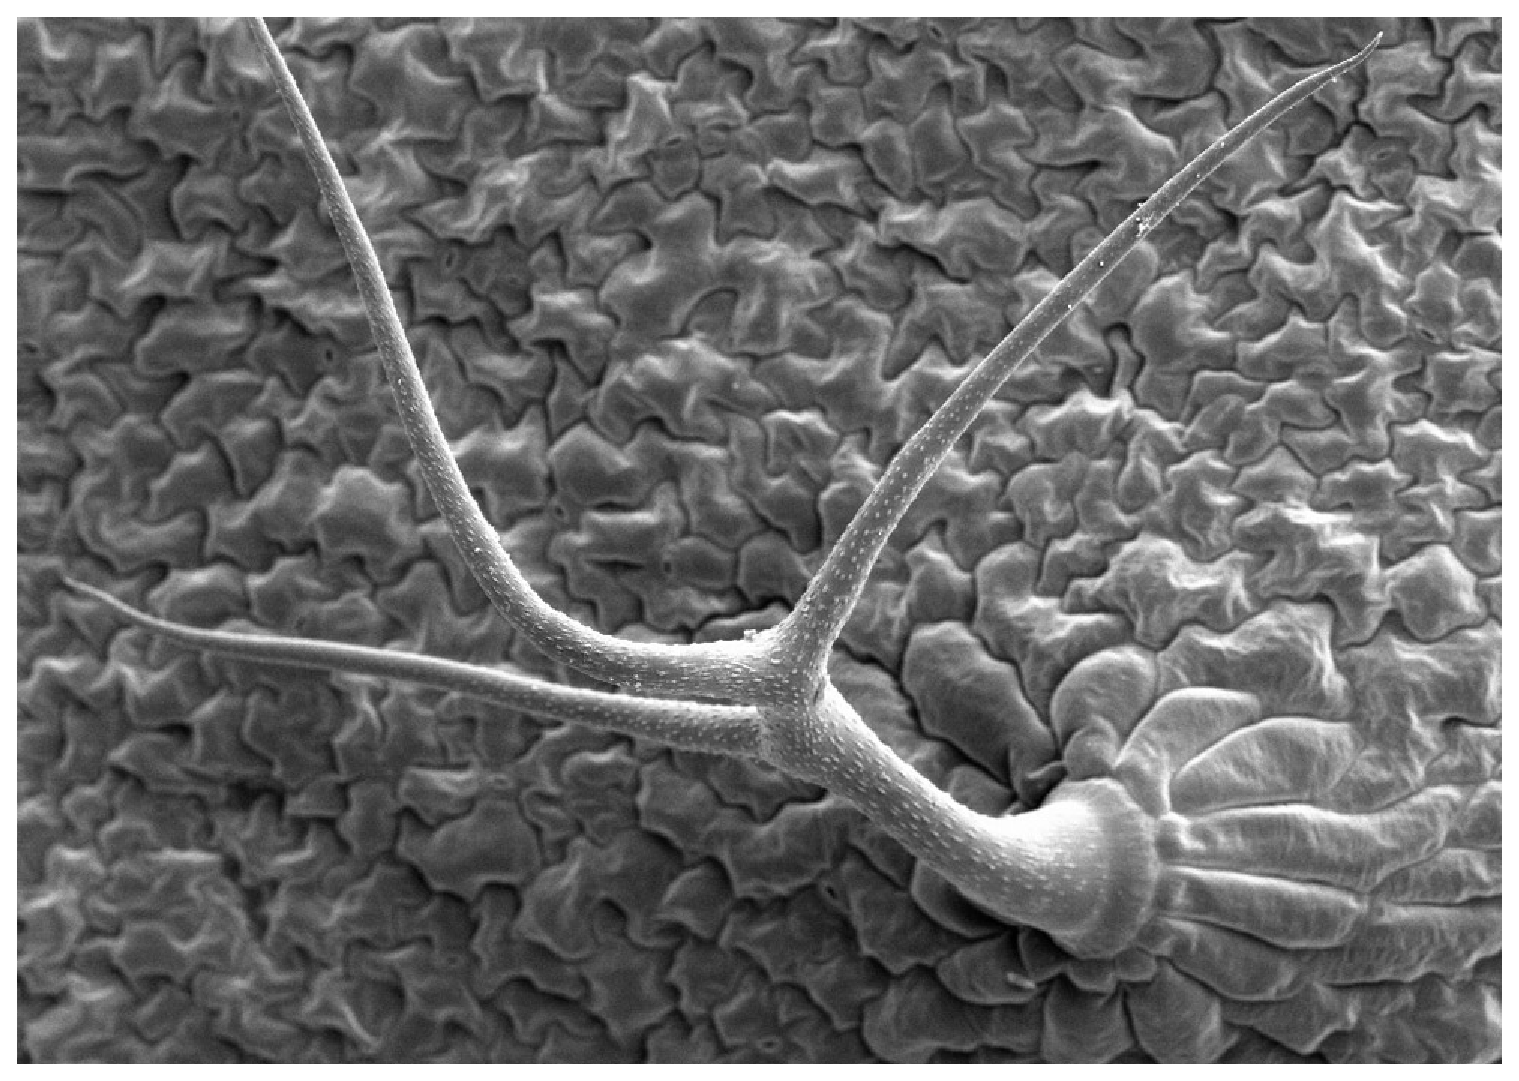
\includegraphics[scale=0.35]{photos/m15_tricome}\label{cacheDados}
\caption{Figura original a ser comparada}
\end{center}
\end{figure}



%m15 fig1
\begin{figure}[h!]
\begin{center}
\subfloat[Sobreposição da palavra CTW na figura original]{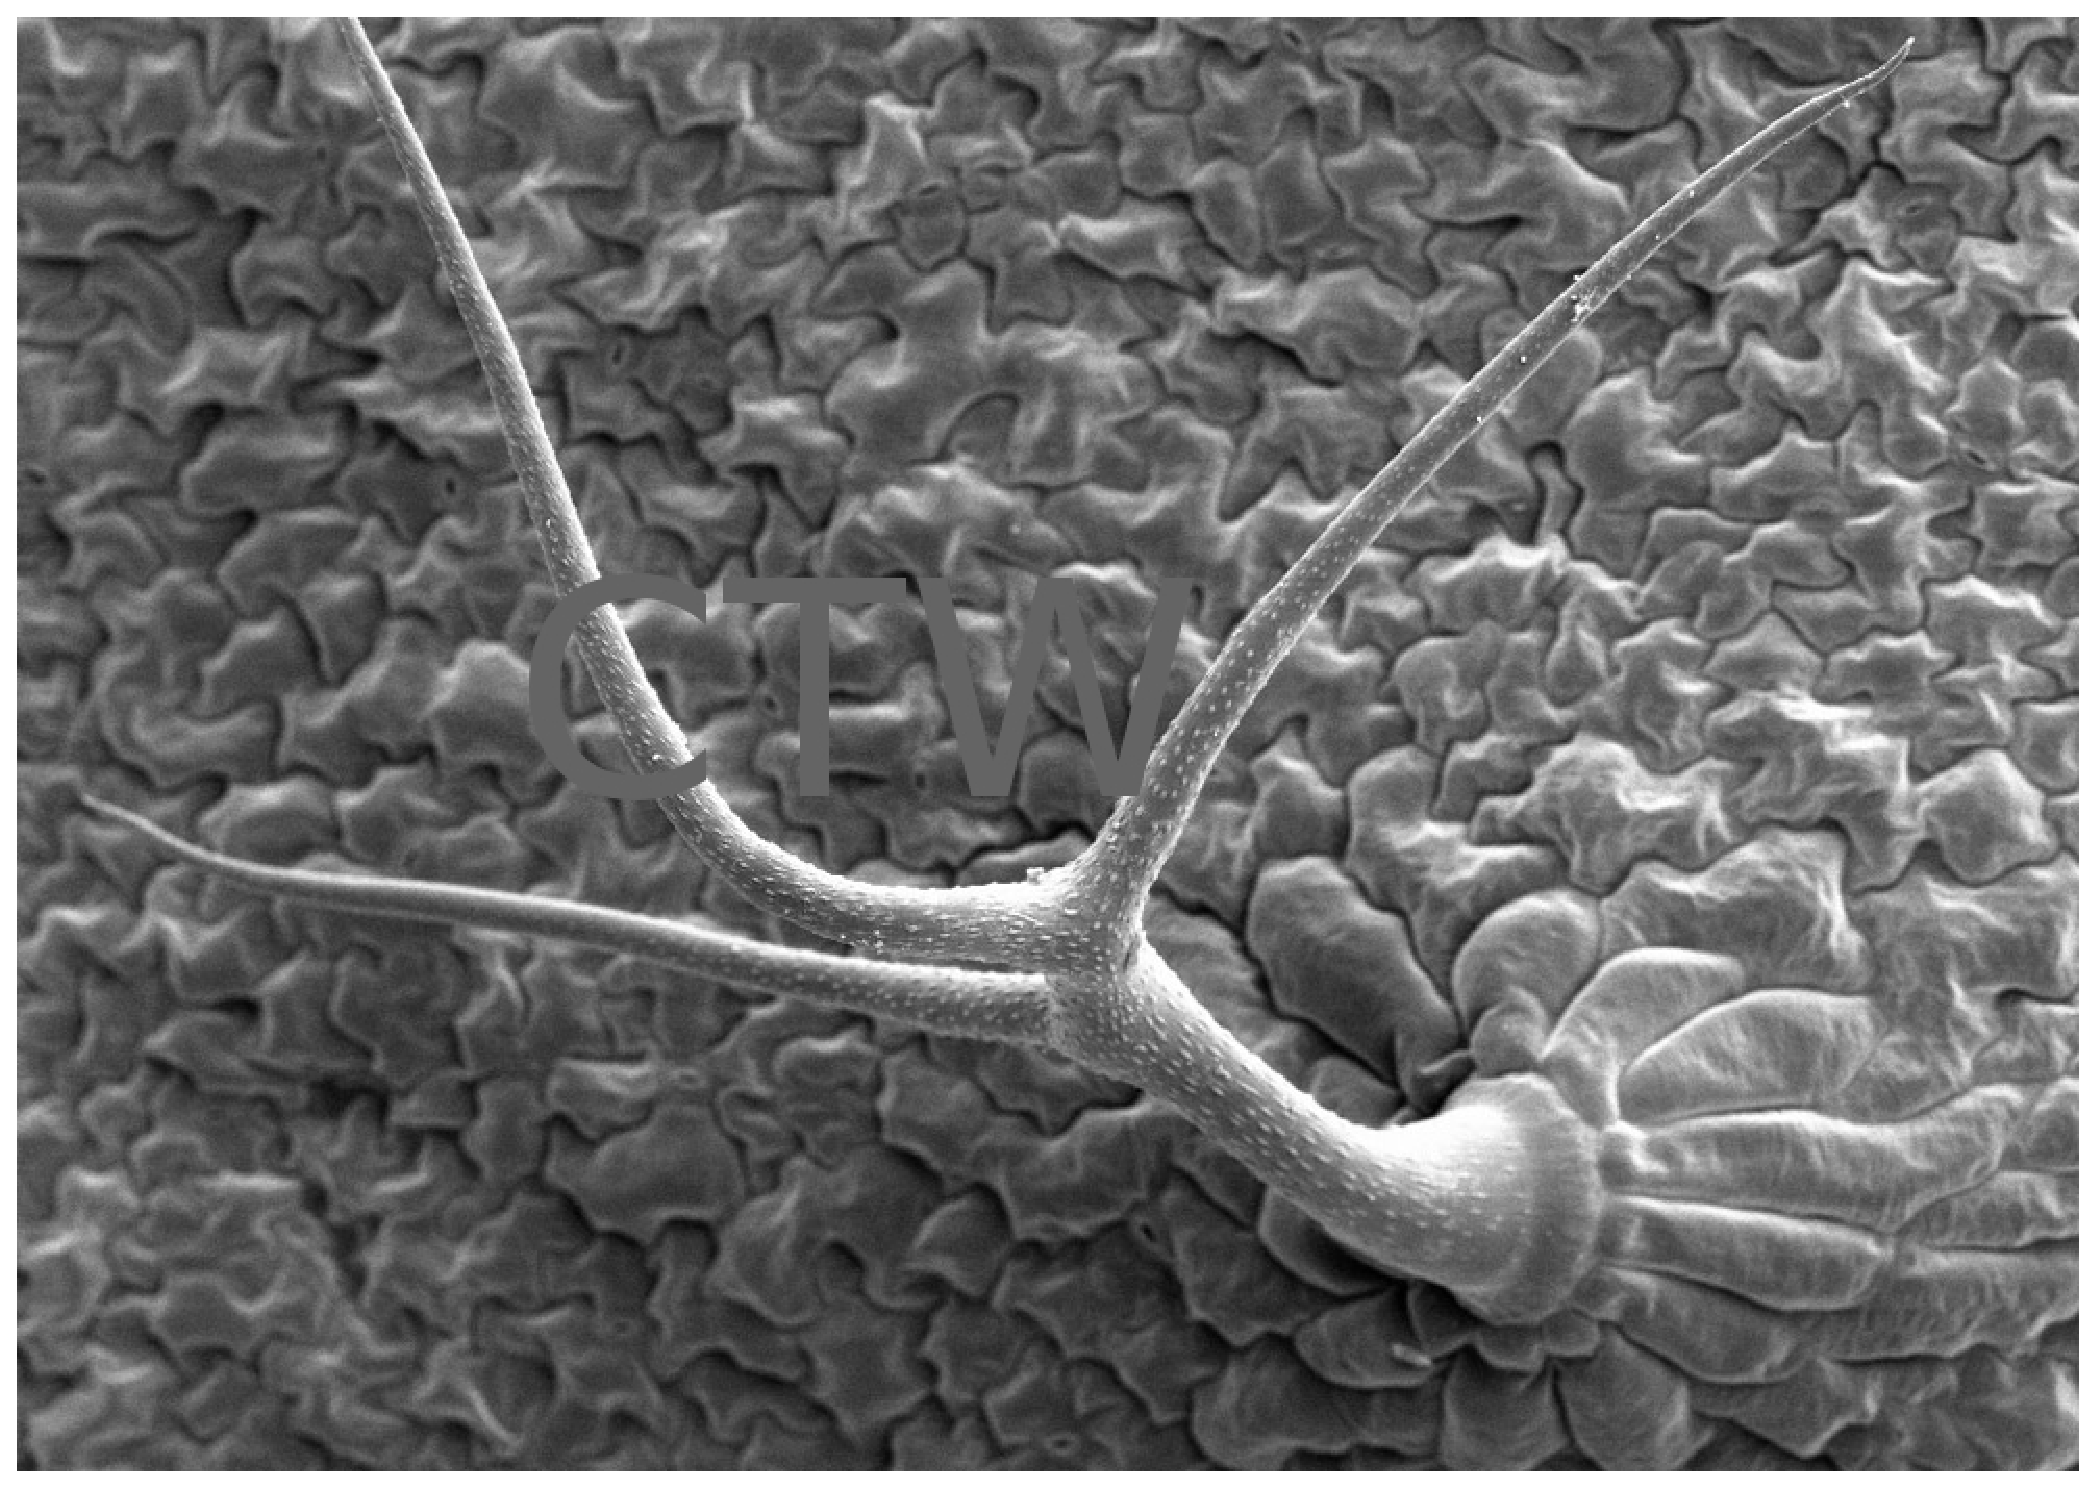
\includegraphics[scale=0.22]{photos/m15_tricome_b}\label{cacheDados}}
\hspace{5mm}
\subfloat[Alterção da posição da palavra CTW ]{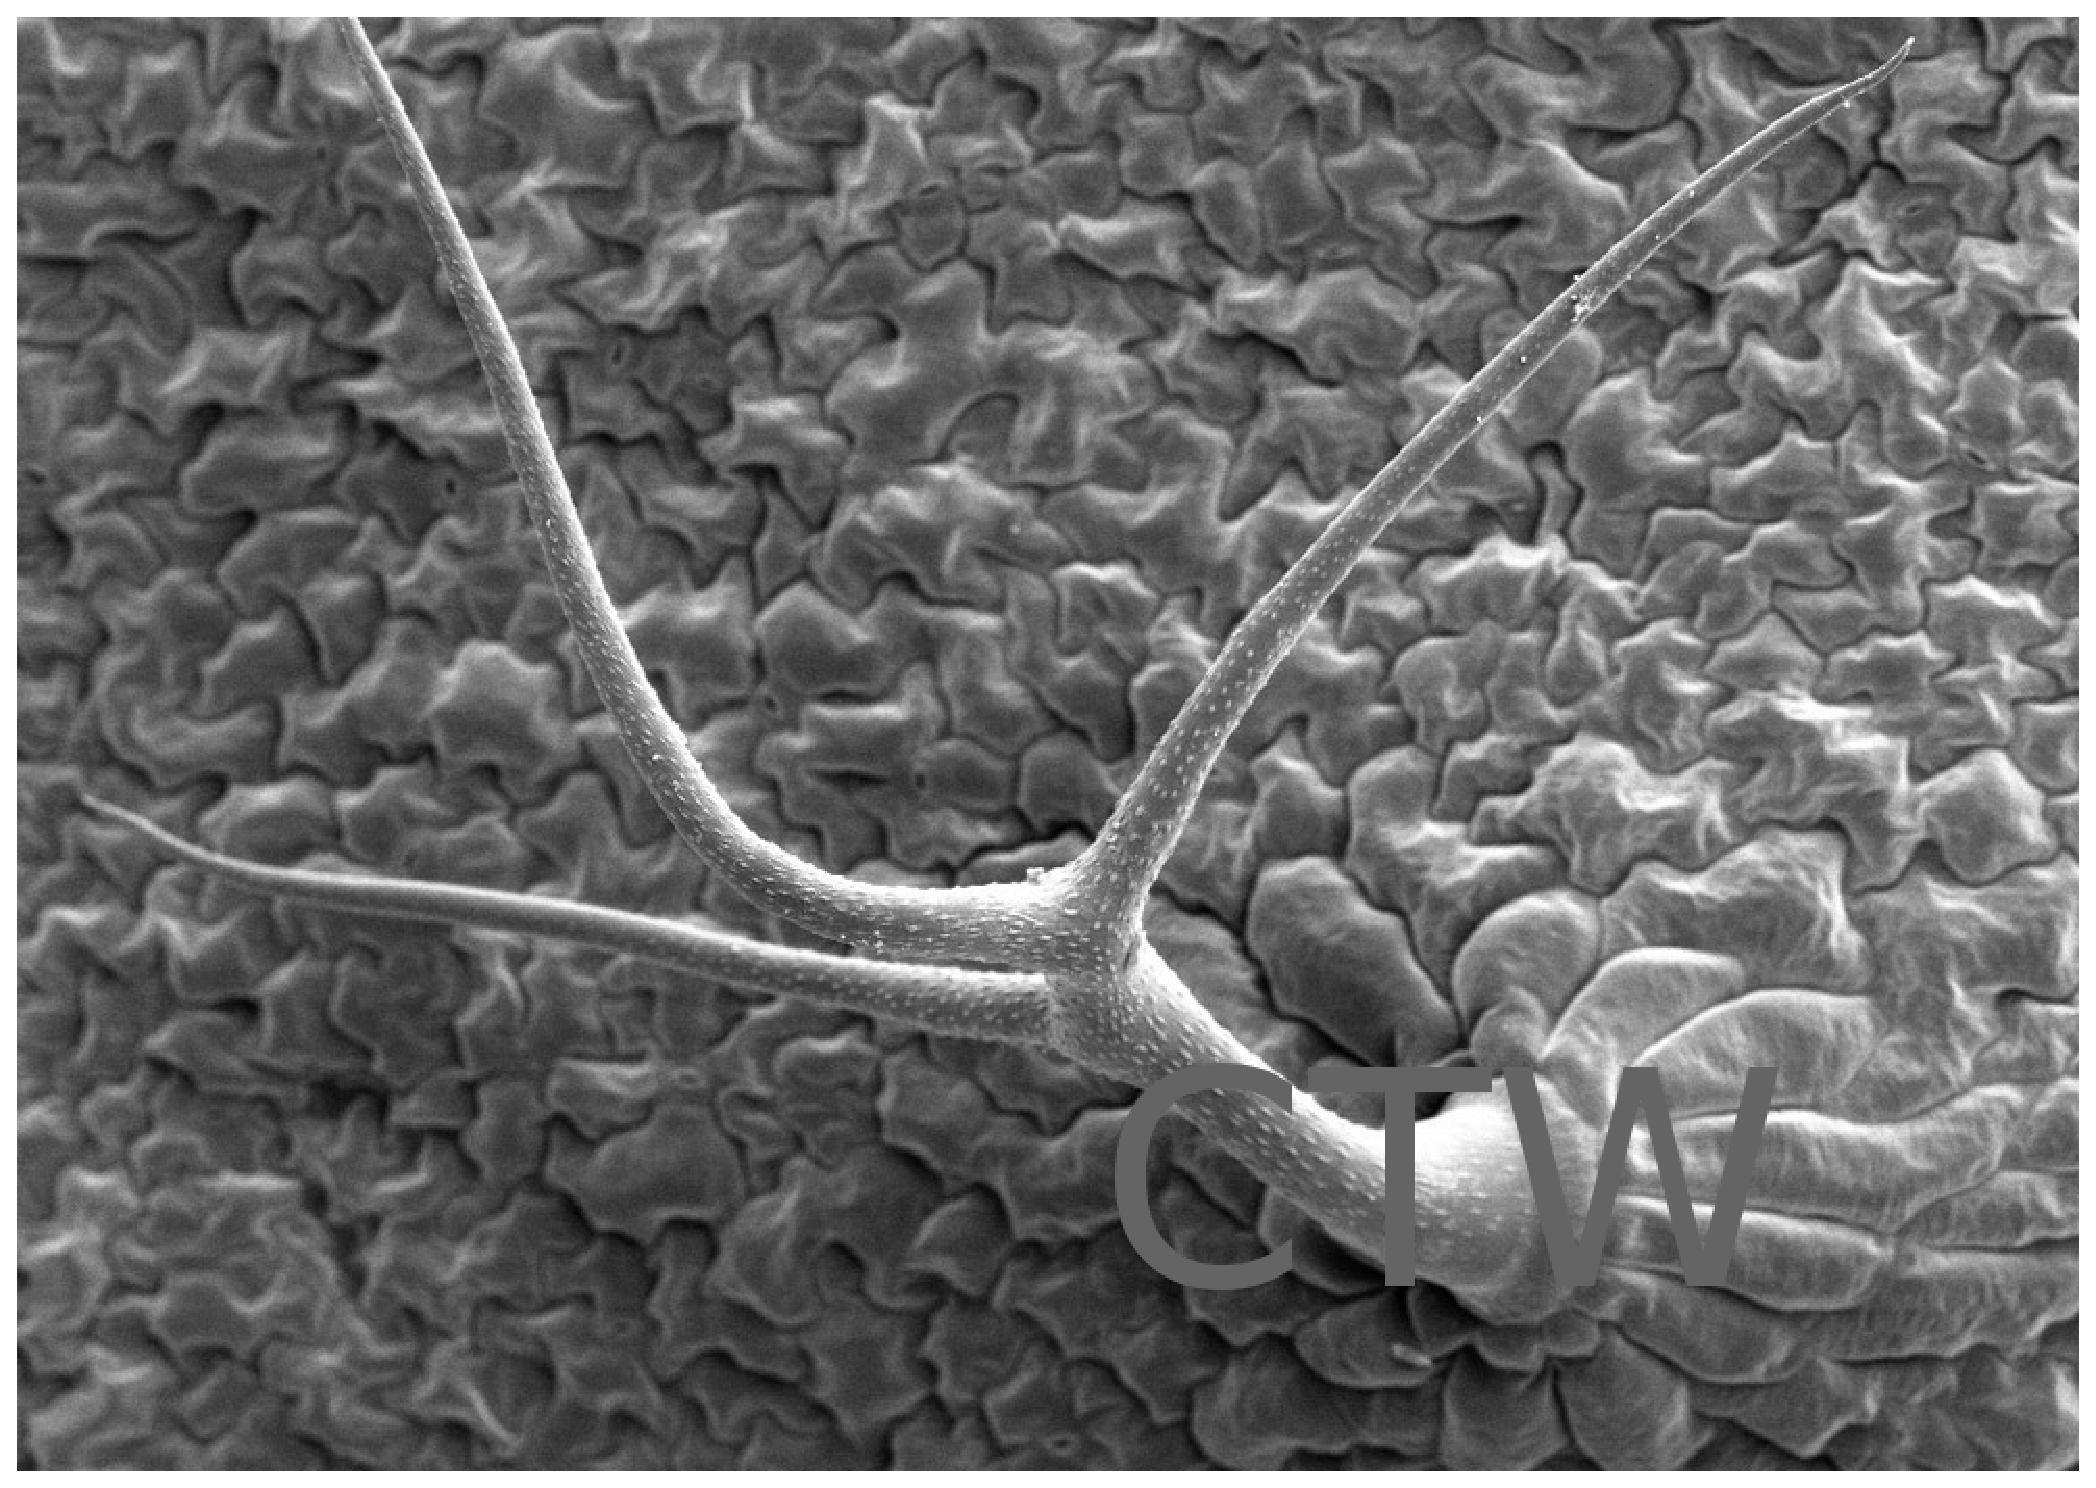
\includegraphics[scale=0.22]{photos/m15_tricome_c}\label{cacheIns}}
\caption{Comparação entre a foto original e duas fotos compostas pela
  sobreposição de uma palavra à imagem original}
\end{center}
\end{figure}

\newpage

%m15 fig1
\begin{figure}[h!]
\begin{center}
\subfloat[Sobreposição da foto de Lena com grau de transparência maior]{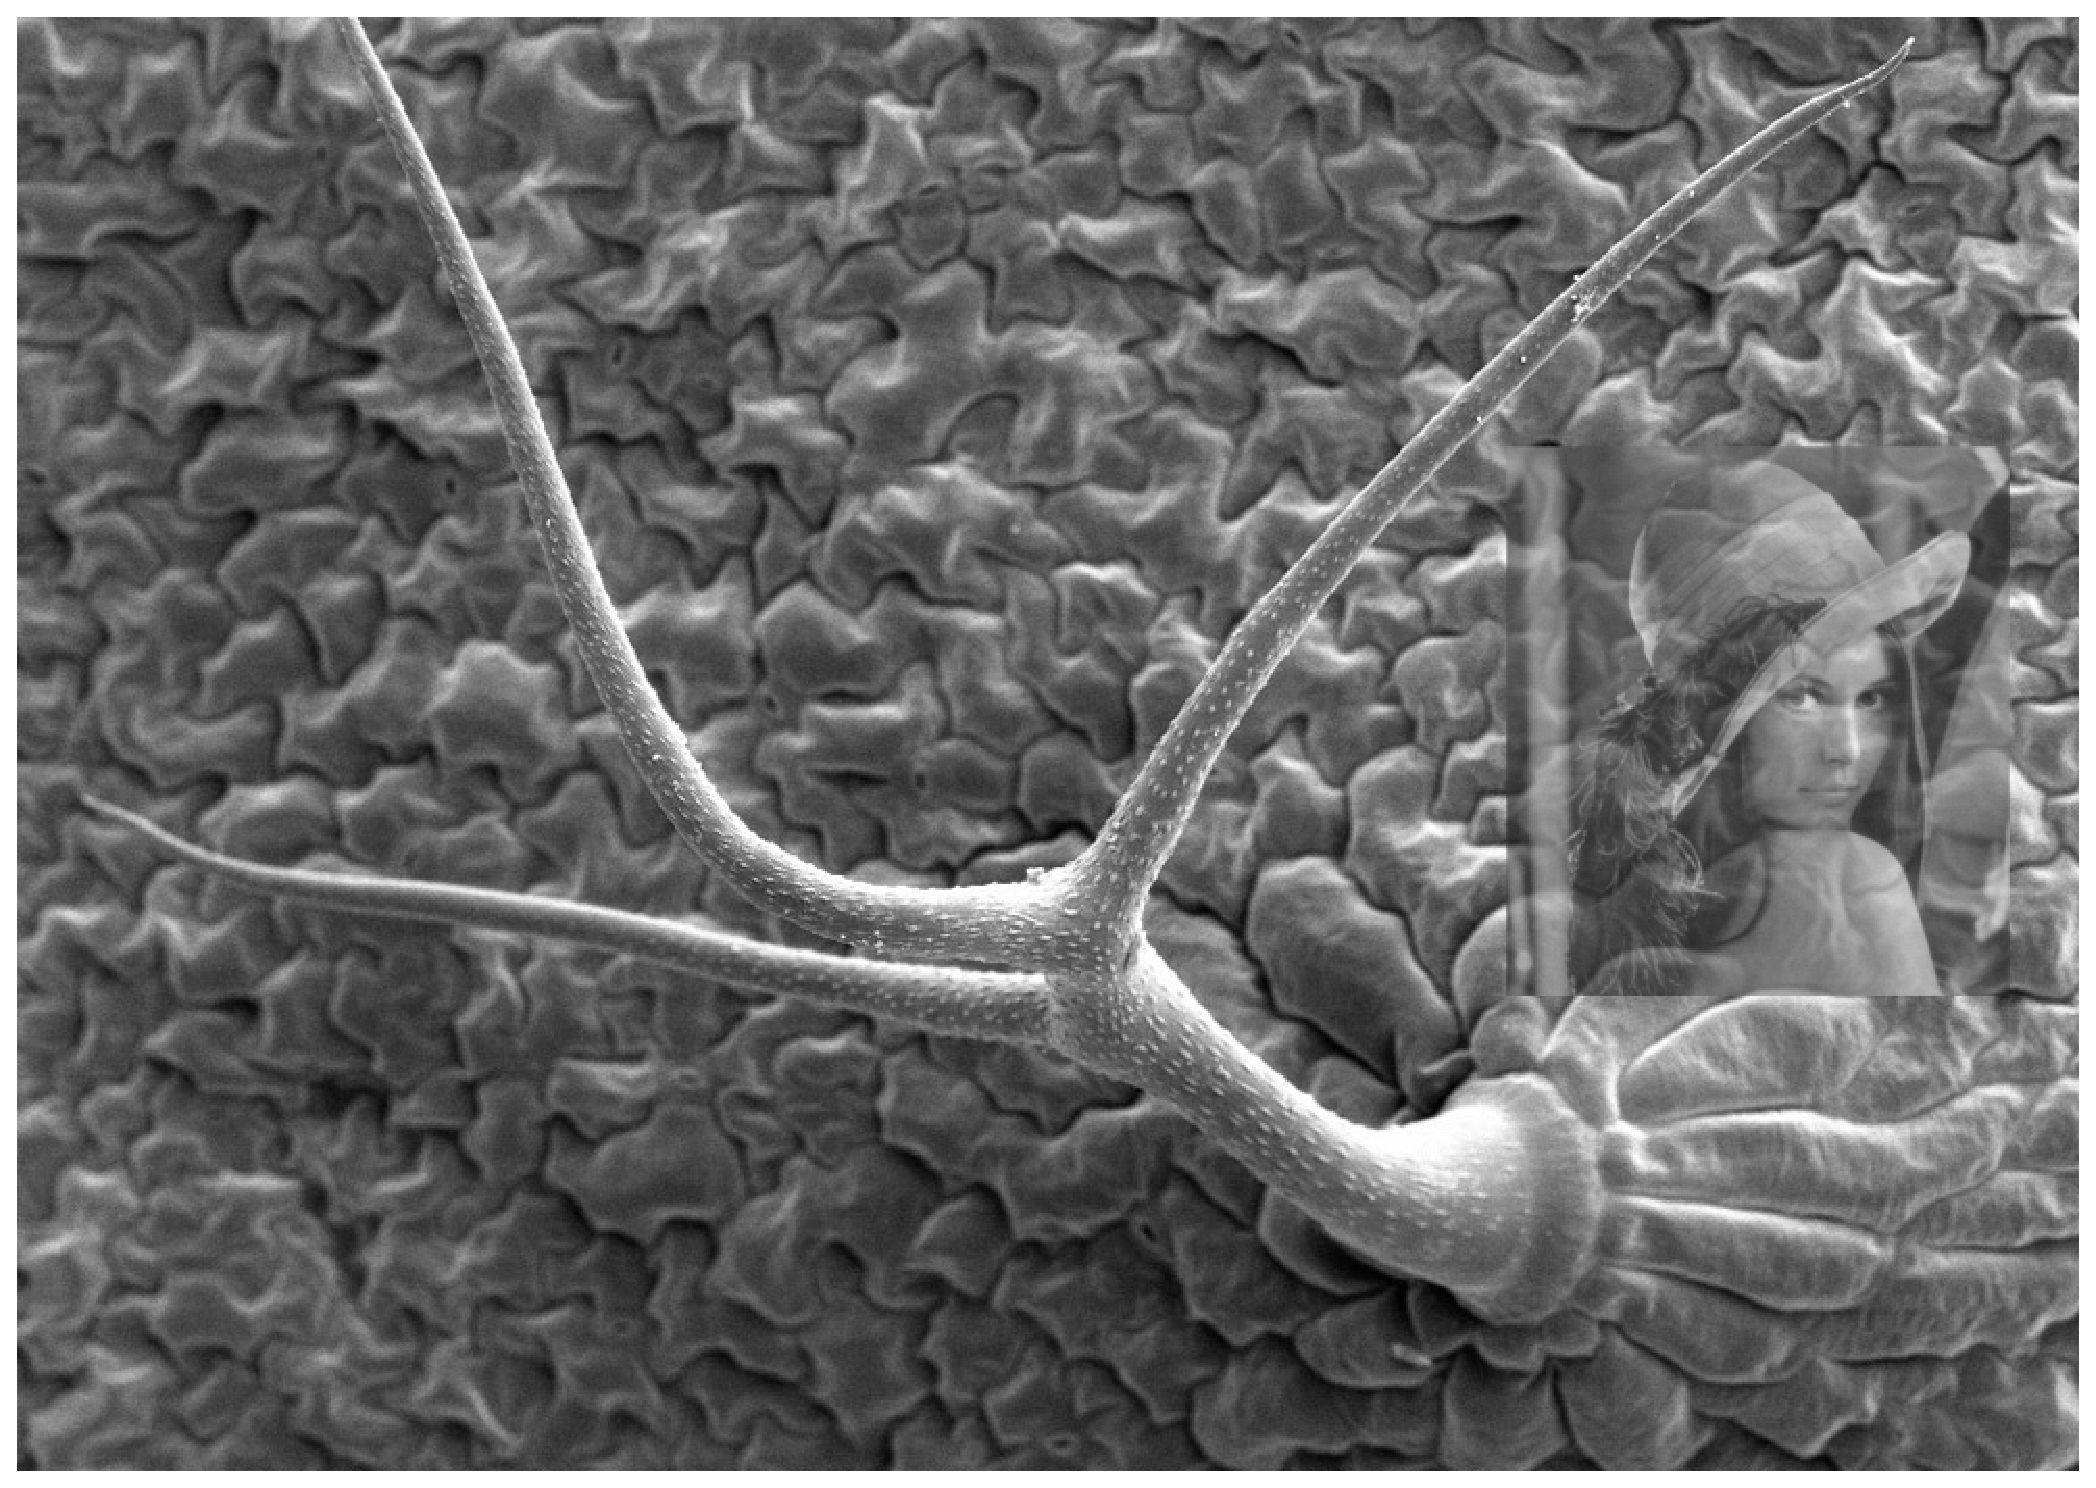
\includegraphics[scale=0.22]{photos/m15_tricome_d}\label{
cacheDados}}
\hspace{10mm}
\subfloat[Sobreposição  da foto de Lena com grau de transparência menor]{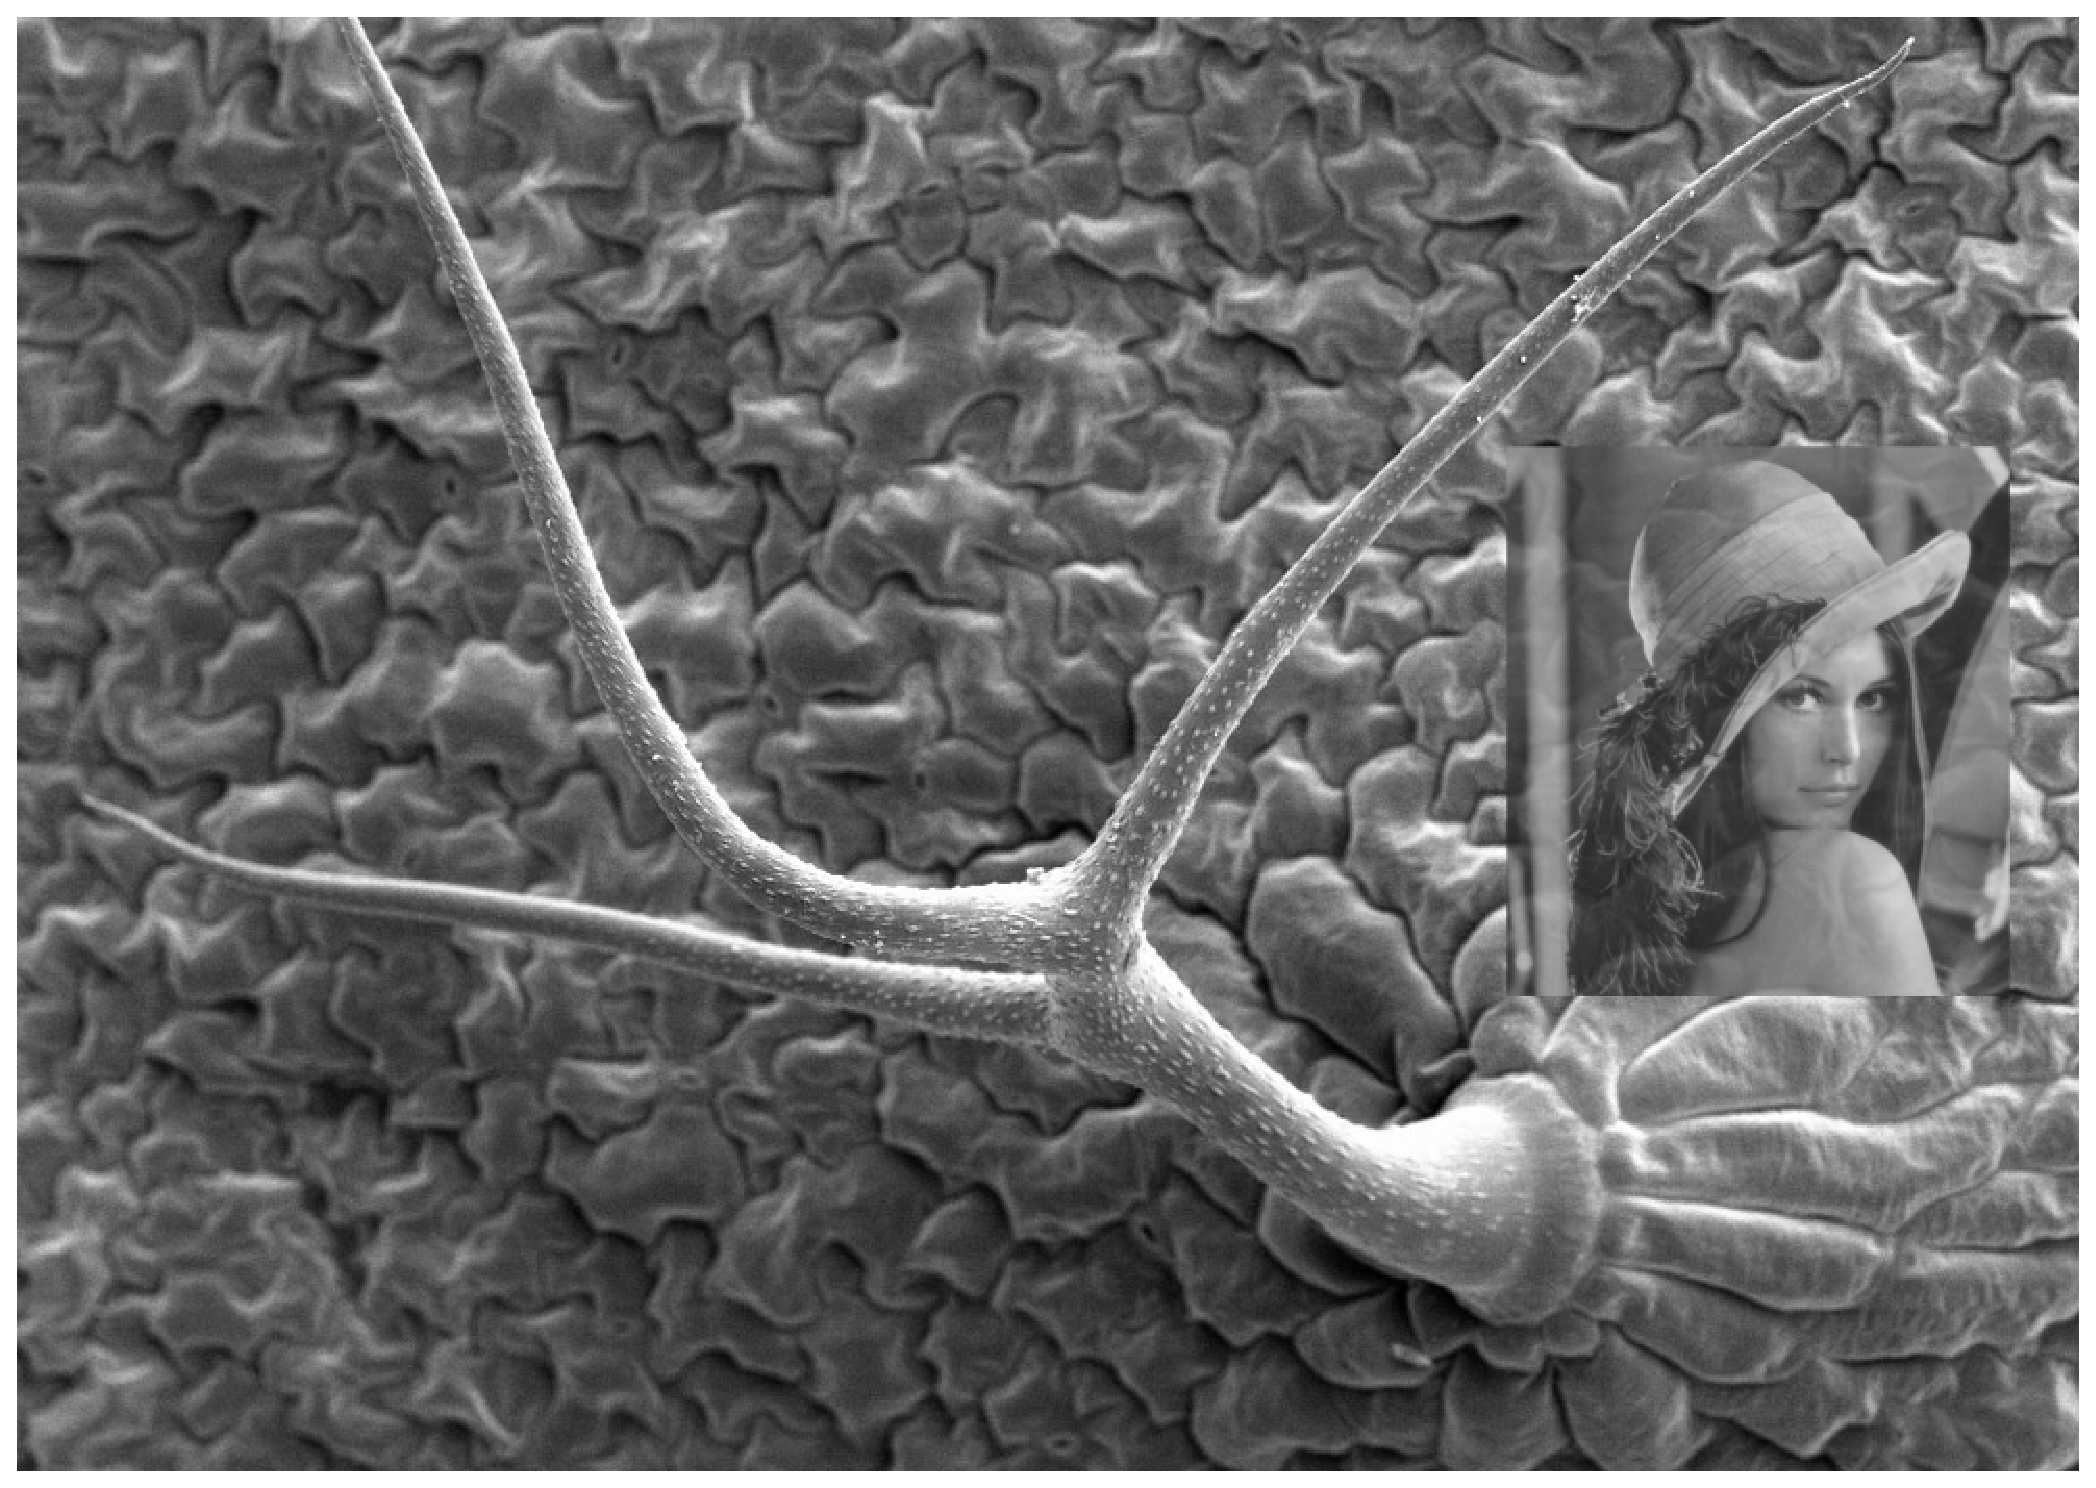
\includegraphics[scale=0.22]{photos/m15_tricome_e}\label{cacheIns}}
\caption{Comparação entre a imagem original e duas imagens compostas pela sobreposição
  de uma outra imagem à imagem original}
\end{center}
\end{figure}



\section{Conclusão}

% ******************************************************
% 		REFERENCIAS BIBLIOGRÁFICAS
% ******************************************************
%\section{Referências}
\bibliographystyle{plain}
\begin{small}
  \bibliography{referencias}
\end{small}

\end{document}
